Ein Markov Descision Process

\begin{figure}[H]
    \centering
    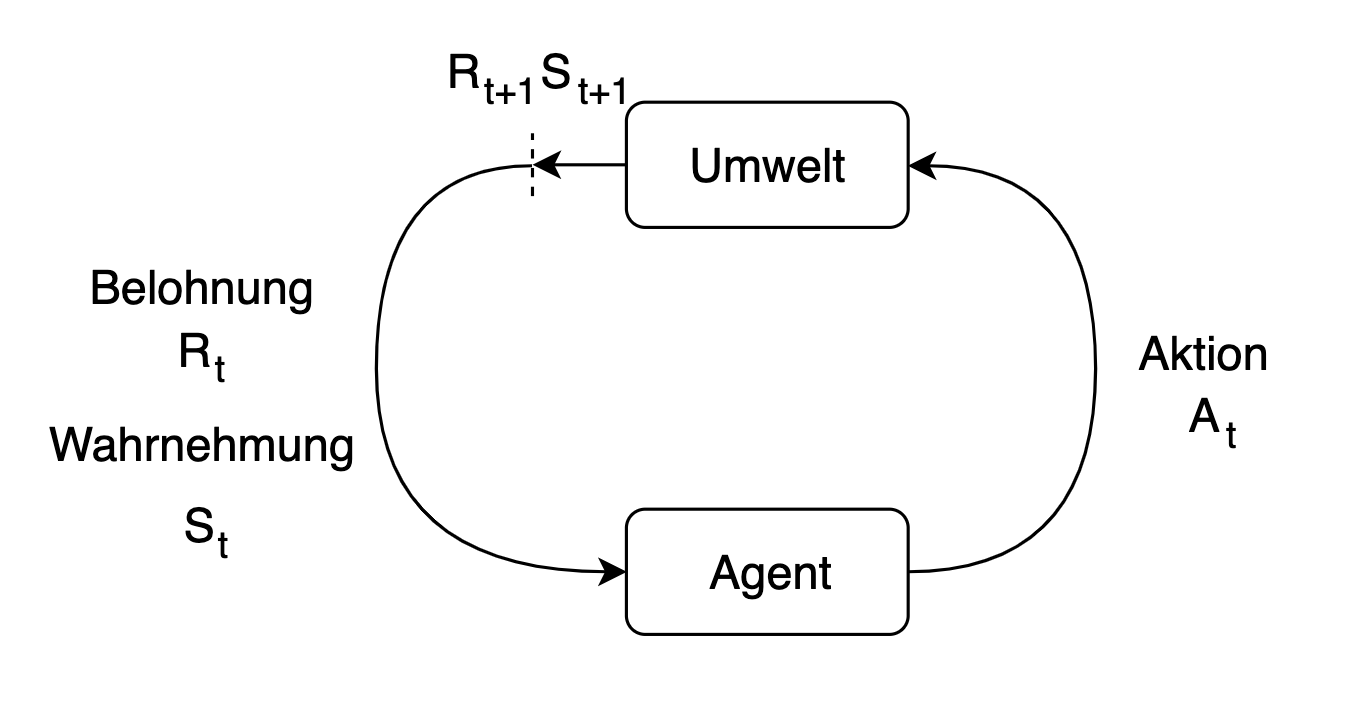
\includegraphics[height=200px]{images/agentUmweltInterface.png}
    \caption{ Agent-Umwelt Interface}
\end{figure}



Der Agent interagiert mit dem MDP jeweils zu diskreten Zeitpunkten $t = 0, 1, 2, 3, ...$. \\
Zu jedem Zeitpunkt $t$ beobachtet der Agent den Zustand seiner Umgebung $S_t \in \mathcal{S}$ und wählt aufgrund dessen eine Aktionen $A_t \in \mathcal{A}$. Als Konsequenz seiner Aktion erhält er einen Zeitpunkt später eine Belohnung $R_{t+1} \in \mathcal{E} \subset\mathbb{R} $ und stellt den Folgezustand $S_{t+1}$ fest. Das Zusammenspiel zwischen Agenten und MDP erzeugt also folgende Reihenfolge:
\[S_0, A_0, R_1, S_1, A_1, R_2, S_2, A_2, R_3, ...\]

